\documentclass[12pt]{article}

\usepackage[a4paper,left=1.5cm,right=1.5cm,top=1.5cm,bottom=1.5cm]{geometry}
\usepackage[T1]{fontenc}
\usepackage[utf8]{inputenc}
\usepackage{lmodern}
\usepackage{amsmath}
\usepackage{amssymb}
\usepackage{array}
\usepackage{tikz}

\usetikzlibrary{arrows.meta}

\setlength{\parindent}{0pt}
\setlength{\parskip}{0pt}
\renewcommand{\arraystretch}{1.35}

\newcommand{\QuestionMarks}[1]{\hfill [#1]}
\newcommand{\AnswerLine}[1]{\makebox[#1]{\hrulefill}}
\newcommand{\AnswerBox}{\fbox{\rule{0pt}{0.8cm}\rule{0.8cm}{0pt}}}

\begin{document}
	
	\textbf{1}\quad
	\textbf{(a)}\quad
	Write six thousand three hundred and twenty four in figures.
	
	\vspace{0.35cm}
	
	\hfill \AnswerLine{7cm} \QuestionMarks{1}
	
	\vspace{0.55cm}
	
	\hspace*{0.8cm}
	\textbf{(b)}\quad
	Write the number 13\,742 in words.
	
	\vspace{0.35cm}
	
	\hfill \AnswerLine{13cm}
	
	\vspace{0.25cm}
	
	\hfill \AnswerLine{13cm} \QuestionMarks{1}
	
	\vspace{0.65cm}
	
	\textbf{2}\quad
	Here are some fractions.
	
	\vspace{0.35cm}
	
	\[
	\frac{1}{7}
	\qquad\qquad\qquad
	\frac{1}{5}
	\qquad\qquad\qquad
	\frac{1}{9}
	\qquad\qquad\qquad
	\frac{1}{6}
	\]
	
	\vspace{0.25cm}
	
	Draw a ring around the \textbf{smallest} fraction. \QuestionMarks{1}
	
	\vspace{0.75cm}
	
	\textbf{3}\quad
	Carlos collects information from children in his class to show the number of pets they have.
	
	\vspace{0.3cm}
	
	Here is the information.
	
	\vspace{0.35cm}
	
	\begin{tabular}{@{}l@{\quad}r@{\hspace{2.4cm}}l@{\quad}r@{\hspace{2.4cm}}l@{\quad}r@{}}
		Oliver & 0 & Carlos & 1 & Yuri & 7 \\
		Mike & 2 & Rajiv & 2 & Hassan & 4 \\
		Pierre & 3 & Ahmed & 0 & Chen & 3
	\end{tabular}
	
	\vspace{0.35cm}
	
	Complete the chart using the information.
	
	\vspace{0.25cm}
	
	\begin{tabular}{|>{\centering\arraybackslash}p{3.2cm}|>{\centering\arraybackslash}p{3.2cm}|>{\centering\arraybackslash}p{3.2cm}|}
		\hline
		\textbf{number of pets} & \textbf{tally} & \textbf{frequency} \\
		\hline
		0--2 & & \rule{0pt}{0.85cm} \\
		\hline
		3--5 & & \rule{0pt}{0.85cm} \\
		\hline
		6--8 & & \rule{0pt}{0.85cm} \\
		\hline
	\end{tabular}
	\QuestionMarks{2}
	
	\vspace{0.8cm}
	
	\textbf{4}\quad
	Here is a list of symbols.
	
	\vspace{0.3cm}
	
	\hspace*{0.8cm}
	\(=\)
	\hspace{1.2cm}
	\(<\)
	\hspace{1.2cm}
	\(>\)
	
	\vspace{0.45cm}
	
	Write one of the symbols in each box to complete each statement.
	
	\vspace{0.35cm}
	
	\hspace*{1.6cm}
	\begin{tabular}{c@{\hspace{0.6cm}}c@{\hspace{0.6cm}}c}
		\(-4\) & \AnswerBox & \(3\) \\[0.35cm]
		\(9\) & \AnswerBox & \(-2\)
	\end{tabular}
	\QuestionMarks{1}
	
	\vspace{0.8cm}
	
	\textbf{5}\quad
	Here is part of a sequence.
	
	\vspace{0.2cm}
	
	\hspace*{1.0cm}
	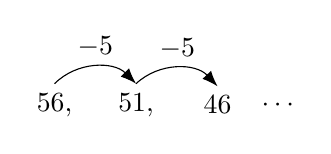
\begin{tikzpicture}[scale=0.9, every node/.style={font=\normalsize}]
		\node (a) at (0,0) {56,};
		\node (b) at (1.15,0) {51,};
		\node (c) at (2.3,0) {46};
		\node (d) at (3.15,0) {\(\cdots\)};
		
		\draw[-{Latex[length=2mm]}, bend left=45] (a.north) to node[above] {\(-5\)} (b.north);
		\draw[-{Latex[length=2mm]}, bend left=45] (b.north) to node[above] {\(-5\)} (c.north);
	\end{tikzpicture}
	
	\vspace{0.25cm}
	
	The sequence continues in the same way.
	
	\vspace{0.35cm}
	
	Write the next two terms in the sequence.
	
	\vspace{0.35cm}
	
	\hfill \AnswerLine{4.4cm}\quad and\quad \AnswerLine{4.4cm} \QuestionMarks{1}
	
	\vspace{0.75cm}
	
	\textbf{6}\quad
	Draw a ring around the number that is divisible by 25
	
	\vspace{0.55cm}
	
	\[
	60
	\qquad\qquad
	65
	\qquad\qquad
	70
	\qquad\qquad
	75
	\qquad\qquad
	80
	\]
	
	\vspace{0.25cm}
	
	\QuestionMarks{1}
	
	\vspace{0.75cm}
	
	\textbf{7}\quad
	Jamila counts on from 16 in steps of 10
	
	\vspace{0.45cm}
	
	\hspace*{1.2cm}
	16
	\hspace{1.3cm}
	26
	\hspace{1.3cm}
	36
	\hspace{1.3cm}
	46
	
	\vspace{0.45cm}
	
	Write down any two numbers between 100 and 130 that Jamila says.
	
	\vspace{0.45cm}
	
	\hfill \AnswerLine{4.4cm}\quad and\quad \AnswerLine{4.4cm} \QuestionMarks{1}
	
	\vspace{0.8cm}
	
	\textbf{8}\quad
	Here is a rectangle.
	
	\vspace{0.35cm}
	
	\begin{center}
		\begin{tikzpicture}[scale=0.85]
			\draw[line width=0.6pt] (0,0) rectangle (5.6,1.8);
		\end{tikzpicture}
	\end{center}
	
	\vspace{0.25cm}
	
	Draw \textbf{all} the lines of symmetry on the rectangle.
	
	Use a ruler. \QuestionMarks{1}
	
	\vspace{0.8cm}
	
	\textbf{9}\quad
	Mia wakes up at 7.00 am on Tuesday and gets ready for school.
	
	\vspace{0.3cm}
	
	Draw a line to match each of the events to the correct likelihood.
	
	\vspace{0.35cm}
	
	\begin{center}
		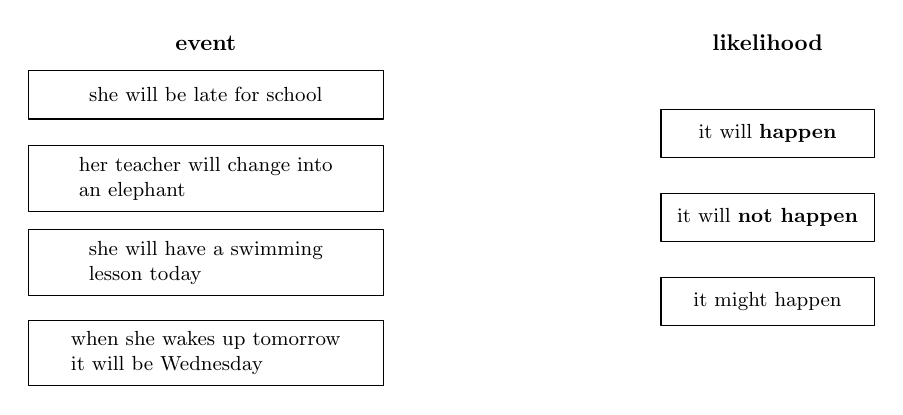
\begin{tikzpicture}[
			scale=0.82,
			every node/.style={font=\small, transform shape},
			line cap=round,
			line join=round
			]
			\node[font=\bfseries] at (2.4,5.15) {event};
			\node[font=\bfseries] at (11.1,5.15) {likelihood};
			
			\node[
			draw,
			minimum width=5.5cm,
			minimum height=0.75cm,
			align=left,
			inner sep=5pt,
			anchor=center
			] at (2.4,4.35) {she will be late for school};
			
			\node[
			draw,
			minimum width=5.5cm,
			minimum height=0.9cm,
			align=left,
			inner sep=5pt,
			anchor=center
			] at (2.4,3.05) {her teacher will change into\\an elephant};
			
			\node[
			draw,
			minimum width=5.5cm,
			minimum height=0.9cm,
			align=left,
			inner sep=5pt,
			anchor=center
			] at (2.4,1.75) {she will have a swimming\\lesson today};
			
			\node[
			draw,
			minimum width=5.5cm,
			minimum height=1.0cm,
			align=left,
			inner sep=5pt,
			anchor=center
			] at (2.4,0.35) {when she wakes up tomorrow\\it will be Wednesday};
			
			\node[
			draw,
			minimum width=3.3cm,
			minimum height=0.75cm,
			align=left,
			inner sep=5pt,
			anchor=center
			] at (11.1,3.75) {it will \textbf{happen}};
			
			\node[
			draw,
			minimum width=3.3cm,
			minimum height=0.75cm,
			align=left,
			inner sep=5pt,
			anchor=center
			] at (11.1,2.45) {it will \textbf{not happen}};
			
			\node[
			draw,
			minimum width=3.3cm,
			minimum height=0.75cm,
			align=left,
			inner sep=5pt,
			anchor=center
			] at (11.1,1.15) {it might happen};
		\end{tikzpicture}
	\end{center}
	
	\QuestionMarks{2}
	
	\vspace{0.8cm}
	
	\textbf{10}\quad
	Here are some angles.
	
	\vspace{0.35cm}
	
	\begin{center}
		\begin{tikzpicture}[
			scale=0.75,
			line cap=round,
			line join=round,
			line width=0.55pt
			]
			
			\def\AngleSideLength{1.70}
			\def\AngleArcRadius{0.58}
			
			\newcommand{\UniformAngle}[2]{%
				\coordinate (O) at (0,0);
				\draw (O) -- (#1:\AngleSideLength);
				\draw (O) -- (#2:\AngleSideLength);
				\draw (O) ++(#1:\AngleArcRadius)
				arc[start angle=#1,end angle=#2,radius=\AngleArcRadius];
			}
			
			% Angle 1
			\begin{scope}[shift={(0,0)}]
				\UniformAngle{162}{139}
			\end{scope}
			
			% Angle 2
			\begin{scope}[shift={(2.7,0.1)}]
				\UniformAngle{-32}{58}
			\end{scope}
			
			% Angle 3
			\begin{scope}[shift={(6.0,0.1)}]
				\UniformAngle{-2}{145}
			\end{scope}
			
			% Angle 4
			\begin{scope}[shift={(9.4,0.05)}]
				\UniformAngle{142}{72}
			\end{scope}
			
			% Angle 5
			\begin{scope}[shift={(12.1,0.05)}]
				\UniformAngle{75}{-34}
			\end{scope}
			
		\end{tikzpicture}
	\end{center}
	
	\vspace{0.3cm}
	
	Draw a ring around \textbf{all} the acute angles. \QuestionMarks{1}
	
	\vspace{0.8cm}
	
	\textbf{11}\quad
	Here are some numbers.
	
	\vspace{0.3cm}
	
	\[
	1
	\qquad\qquad
	4
	\qquad\qquad
	5
	\qquad\qquad
	8
	\qquad\qquad
	12
	\]
	
	\vspace{0.2cm}
	
	\begin{center}
		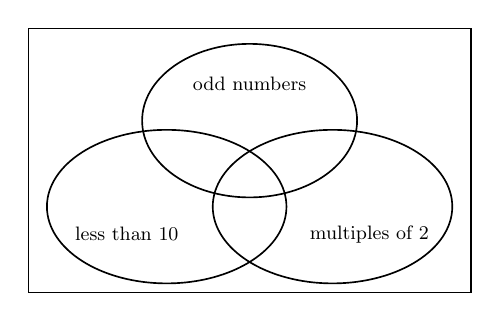
\begin{tikzpicture}[
			scale=0.78,
			every node/.style={font=\small, transform shape}
			]
			\draw[line width=0.6pt] (-3.6,-2.05) rectangle (3.6,2.25);
			
			\draw[line width=0.6pt] (0,0.75) ellipse (1.75 and 1.25);
			\draw[line width=0.6pt] (-1.35,-0.65) ellipse (1.95 and 1.25);
			\draw[line width=0.6pt] (1.35,-0.65) ellipse (1.95 and 1.25);
			
			\node at (0,1.35) {odd numbers};
			\node at (-2.0,-1.1) {less than 10};
			\node at (1.95,-1.1) {multiples of 2};
		\end{tikzpicture}
	\end{center}
	
	Write the numbers in the correct place on the Venn diagram. \QuestionMarks{2}
	
	\vspace{0.8cm}
	
	\textbf{12}\quad
	Here is a rectangle.
	
	\vspace{0.25cm}
	
	\hspace*{0.8cm}
	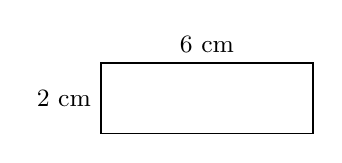
\begin{tikzpicture}[
		x=0.45cm,
		y=0.45cm,
		every node/.style={font=\small}
		]
		\draw[line width=0.6pt] (0,0) rectangle (6,2);
		\node[above] at (3,2) {6 cm};
		\node[left] at (0,1) {2 cm};
	\end{tikzpicture}
	
	\vspace{0.35cm}
	
	Two of these rectangles are joined to make a new shape.
	
	\vspace{0.25cm}
	
	\hspace*{0.8cm}
	\begin{tikzpicture}[
		x=0.45cm,
		y=0.45cm,
		every node/.style={font=\small}
		]
		
		\def\RectLong{6}
		\def\RectShort{2}
		
		% First copy of the 6 cm by 2 cm rectangle, placed horizontally.
		\draw[line width=0.6pt]
		(0,\RectLong) rectangle (\RectLong,{\RectLong+\RectShort});
		
		% Second copy of the same 6 cm by 2 cm rectangle, rotated vertically.
		\draw[line width=0.6pt]
		(0,0) rectangle (\RectShort,\RectLong);
		
	\end{tikzpicture}
	
	\vspace{0.35cm}
	
	Calculate the area of the new shape.
	
	\vspace{0.45cm}
	
	\hfill \AnswerLine{4.5cm}\quad cm\(^{2}\) \QuestionMarks{1}
	
	\vspace{0.8cm}
	
	\textbf{13}\quad
	Six children share one pizza equally.
	
	\vspace{0.3cm}
	
	Draw a ring around the number statement which shows the fraction of pizza each child gets.
	
	\vspace{0.45cm}
	
	\[
	1 \div 6 = \frac{6}{1}
	\qquad\qquad
	1 \div 6 = \frac{1}{6}
	\qquad\qquad
	6 \div 1 = \frac{6}{1}
	\qquad\qquad
	6 \div 1 = \frac{1}{6}
	\]
	
	\vspace{0.2cm}
	
	\QuestionMarks{1}
	
	\vspace{0.8cm}
	
	\textbf{14}\quad
	Aiko sorts some numbers into groups of odd numbers and even numbers.
	
	\vspace{0.25cm}
	
	\begin{center}
		\begin{tabular}{|>{\centering\arraybackslash}p{4.6cm}|>{\centering\arraybackslash}p{4.6cm}|}
			\hline
			\textbf{odd numbers} & \textbf{even numbers} \\
			\hline
			\rule{0pt}{0.8cm}253 \hspace{1.1cm} 567 & 450 \hspace{1.1cm} 976 \\
			\rule{0pt}{0.8cm}134 \hspace{1.1cm} 761 & 852 \hspace{1.1cm} 654 \\
			\hline
		\end{tabular}
	\end{center}
	
	\vspace{0.25cm}
	
	Draw a ring around the number that is \textbf{not} in the correct place.
	
	\vspace{0.25cm}
	
	Explain how you know.
	
	\vspace{0.25cm}
	
	\AnswerLine{16cm}
	
	\vspace{0.25cm}
	
	\AnswerLine{16cm}
	
	\vspace{0.25cm}
	
	\AnswerLine{16cm} \QuestionMarks{1}
	
	\vspace{0.8cm}
	
	\textbf{15}\quad
	Here are some measurements.
	
	\vspace{0.25cm}
	
	\begin{center}
		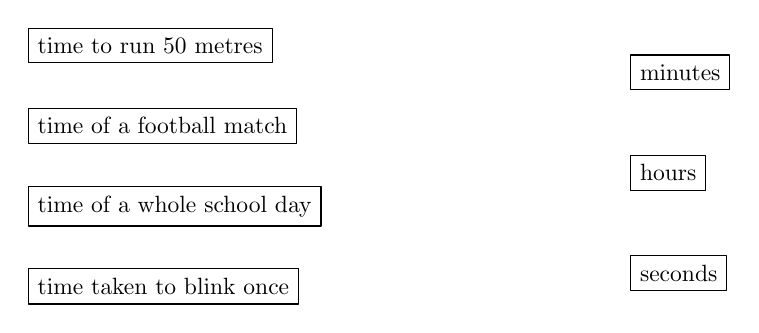
\begin{tikzpicture}[
			scale=0.85,
			every node/.style={font=\normalsize, transform shape},
			line cap=round,
			line join=round
			]
			\node[anchor=west, draw, rectangle, inner sep=4pt] (a1) at (0,3.6) {time to run 50 metres};
			\node[anchor=west, draw, rectangle, inner sep=4pt] (a2) at (0,2.4) {time of a football match};
			\node[anchor=west, draw, rectangle, inner sep=4pt] (a3) at (0,1.2) {time of a whole school day};
			\node[anchor=west, draw, rectangle, inner sep=4pt] (a4) at (0,0.0) {time taken to blink once};
			
			\node[anchor=west, draw, rectangle, inner sep=4pt] (b1) at (9.0,3.2) {minutes};
			\node[anchor=west, draw, rectangle, inner sep=4pt] (b2) at (9.0,1.7) {hours};
			\node[anchor=west, draw, rectangle, inner sep=4pt] (b3) at (9.0,0.2) {seconds};
		\end{tikzpicture}
	\end{center}
	
	\vspace{0.25cm}
	
	Draw a line to connect each measurement to the correct unit they would be measured in. \QuestionMarks{2}
	
	\vspace{0.8cm}
	
	\textbf{16}\quad
	Here is the plan of a park on a grid of squares.
	
	\vspace{0.25cm}
	
	\begin{center}
		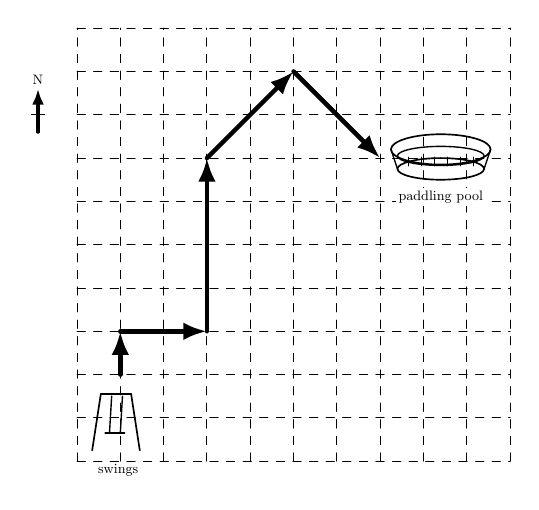
\begin{tikzpicture}[
			scale=0.55,
			every node/.style={font=\small, transform shape},
			line cap=round,
			line join=round
			]
			% North arrow
			\node at (-0.9,8.8) {N};
			\draw[-{Latex[length=2mm]}, line width=1.2pt] (-0.9,7.6) -- (-0.9,8.6);
			\draw[line width=0.5pt] (-1.05,8.0) -- (-0.75,8.0);
			
			% Grid
			\draw[step=1, dashed, line width=0.35pt] (0,0) grid (10,10);
			
			% Path from swings to paddling pool
			\coordinate (P0) at (1,2);
			\coordinate (P1) at (1,3);
			\coordinate (P2) at (3,3);
			\coordinate (P3) at (3,7);
			\coordinate (P4) at (5,9);
			\coordinate (P5) at (7,7);
			
			\draw[-{Latex[length=3mm]}, line width=1.6pt] (P0) -- (P1);
			\draw[-{Latex[length=3mm]}, line width=1.6pt] (P1) -- (P2);
			\draw[-{Latex[length=3mm]}, line width=1.6pt] (P2) -- (P3);
			\draw[-{Latex[length=3mm]}, line width=1.6pt] (P3) -- (P4);
			\draw[-{Latex[length=3mm]}, line width=1.6pt] (P4) -- (P5);
			
			% Swings
			\draw[line width=0.6pt] (0.35,0.25) -- (0.55,1.55);
			\draw[line width=0.6pt] (1.45,0.25) -- (1.25,1.55);
			\draw[line width=0.6pt] (0.55,1.55) -- (1.25,1.55);
			\draw[line width=0.5pt] (0.8,1.5) -- (0.75,0.65);
			\draw[line width=0.5pt] (1.05,1.5) -- (1.0,0.65);
			\draw[line width=0.5pt] (0.65,0.65) -- (1.1,0.65);
			\node[below] at (0.95,0.05) {swings};
			
			% Paddling pool
			\begin{scope}[shift={(8.4,7.2)}]
				\draw[line width=0.6pt] (0,0) ellipse (1.15 and 0.35);
				\draw[line width=0.5pt] (0,-0.15) ellipse (1.0 and 0.22);
				\draw[line width=0.5pt] (-1.15,0) -- (-1.0,-0.45);
				\draw[line width=0.5pt] (1.15,0) -- (1.0,-0.45);
				\draw[line width=0.6pt] (0,-0.45) ellipse (1.0 and 0.25);
				\foreach \x in {-0.75,-0.45,-0.15,0.15,0.45,0.75}
				\draw[line width=0.35pt] (\x,-0.18) -- (\x,-0.38);
			\end{scope}
			\node[fill=white, inner sep=2pt] at (8.4,6.1) {paddling pool};
		\end{tikzpicture}
	\end{center}
	
	\vspace{0.25cm}
	
	Eva walks on paths from the swings to the paddling pool.
	
	The arrows show the direction Eva walks along each path.
	
	\vspace{0.35cm}
	
	Complete the direction Eva walks along each path.
	
	\vspace{0.35cm}
	
	The first one has been done for you.
	
	\vspace{0.25cm}
	
	\begin{tabular}{|>{\centering\arraybackslash}p{4.6cm}|}
		\hline
		\textbf{direction Eva walks along}\\
		\textbf{each path} \\
		\hline
		north \\
		\hline
		\rule{0pt}{0.75cm} \\
		\hline
		\rule{0pt}{0.75cm} \\
		\hline
		\rule{0pt}{0.75cm} \\
		\hline
		\rule{0pt}{0.75cm} \\
		\hline
	\end{tabular}
	
	\QuestionMarks{1}
	
	\vspace{0.8cm}
	
	\textbf{17}\quad
	Darius eats some of a chocolate bar.
	
	The remainder of the chocolate bar is shown on a grid of centimetre squares.
	
	\vspace{0.25cm}
	
	\begin{center}
		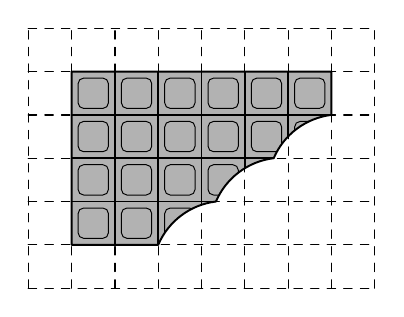
\begin{tikzpicture}[
			scale=0.55,
			line cap=round,
			line join=round
			]
			% Grid of centimetre squares: 8 by 6
			\draw[step=1, dashed, line width=0.45pt] (0,0) grid (8,6);
			
			% Chocolate shape after cutting away everything under 3 arcs
			\begin{scope}
				\clip
				(1,1) --
				(1,5) --
				(7,5) --
				(7,4)
				arc[start angle=96.87,end angle=156.87,radius=5/3]
				arc[start angle=96.87,end angle=156.87,radius=5/3]
				arc[start angle=96.87,end angle=156.87,radius=5/3]
				-- cycle;
				
				% Chocolate fill
				\fill[gray!60] (1,1) rectangle (7,5);
				
				% Chocolate square grid
				\draw[line width=0.6pt] (1,1) grid (7,5);
				
				% Rounded chocolate pieces
				\foreach \x in {1,...,6}
				\foreach \y in {1,...,4}
				{
					\draw[line width=0.35pt, rounded corners=2pt]
					(\x+0.15,\y+0.15) rectangle (\x+0.85,\y+0.85);
				}
			\end{scope}
			
			% Chocolate outline after removing the lower part
			\draw[line width=0.7pt]
			(1,1) --
			(1,5) --
			(7,5) --
			(7,4)
			arc[start angle=96.87,end angle=156.87,radius=5/3]
			arc[start angle=96.87,end angle=156.87,radius=5/3]
			arc[start angle=96.87,end angle=156.87,radius=5/3]
			-- cycle;
		\end{tikzpicture}
	\end{center}
	
	\vspace{0.25cm}
	
	Estimate the area of the remainder of the chocolate bar.
	
	\vspace{0.45cm}
	
	\hfill \AnswerLine{4.5cm}\quad cm\(^{2}\) \QuestionMarks{1}
	
	\vspace{0.8cm}
	
	\textbf{18}\quad
	Arun leaves for a school trip on Monday at 8.00 am.
	
	He returns in the same week on Friday at 5.00 pm.
	
	\vspace{0.35cm}
	
	Calculate the total number of hours for Arun's trip.
	
	\vspace{0.6cm}
	
	\hfill \AnswerLine{4.5cm}\quad hours \QuestionMarks{1}
	
	\vspace{0.8cm}
	
	\textbf{19}\quad
	Here is a list of symbols.
	
	\vspace{0.25cm}
	
	\hspace*{0.8cm}
	\(=\)
	\hspace{1.2cm}
	\(>\)
	\hspace{1.2cm}
	\(<\)
	
	\vspace{0.35cm}
	
	Write one of the symbols in each box to complete each statement.
	
	\vspace{0.3cm}
	
	\hspace*{1.1cm}
	\begin{tabular}{c@{\hspace{0.55cm}}c@{\hspace{0.55cm}}c}
		\(\dfrac{8}{15}\) & \AnswerBox & \(\dfrac{3}{5}\) \\[0.35cm]
		\(\dfrac{8}{20}\) & \AnswerBox & \(\dfrac{4}{10}\)
	\end{tabular}
	\QuestionMarks{1}
	
	\vspace{0.8cm}
	
	\textbf{20}\quad
	Rajiv collects 82 eggs.
	
	\vspace{0.25cm}
	
	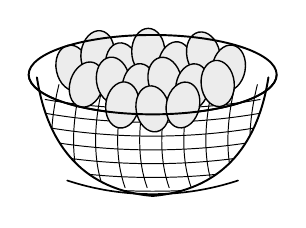
\begin{tikzpicture}[
		scale=0.70,
		every node/.style={font=\small, transform shape},
		line cap=round,
		line join=round
		]
		% =========================
		% Basket outline parameters
		% =========================
		\def\Rx{2.25}
		\def\Ry{0.72}
		
		% --------------------------------
		% Back part of the basket rim
		% --------------------------------
		\draw[line width=0.6pt]
		(-\Rx,0) arc[
		start angle=180,
		end angle=360,
		x radius=\Rx,
		y radius=\Ry
		];
		
		% --------------------------------
		% Basket body
		% --------------------------------
		\draw[line width=0.7pt]
		(-2.1,-0.05)
		.. controls (-1.9,-1.35) and (-1.2,-2.1) .. (0,-2.2)
		.. controls (1.2,-2.1) and (1.9,-1.35) .. (2.1,-0.05);
		
		\draw[line width=0.6pt]
		(-1.55,-1.92)
		.. controls (-0.55,-2.25) and (0.55,-2.25) .. (1.55,-1.92);
		
		% --------------------------------
		% Basket weave, clipped to body
		% --------------------------------
		\begin{scope}
			\clip
			(-2.1,-0.05)
			.. controls (-1.9,-1.35) and (-1.2,-2.1) .. (0,-2.2)
			.. controls (1.2,-2.1) and (1.9,-1.35) .. (2.1,-0.05)
			-- cycle;
			
			\foreach \y in {-0.45,-0.70,-0.95,-1.20,-1.45,-1.70,-1.95}
			{
				\draw[line width=0.35pt]
				(-1.95,\y)
				.. controls (-0.7,\y-0.22) and (0.7,\y-0.22) .. (1.95,\y);
			}
			
			\foreach \x in {-1.7,-1.3,-0.9,-0.5,-0.1,0.3,0.7,1.1,1.5,1.9}
			{
				\draw[line width=0.35pt]
				(\x,-0.18)
				.. controls (\x-0.18,-0.9) and (\x-0.18,-1.55) .. (\x,-2.05);
			}
		\end{scope}
		
		% --------------------------------
		% Eggs
		% --------------------------------
		\foreach \x/\y/\ang in {
			-1.45/0.12/12,
			-1.00/0.38/-8,
			-0.55/0.16/10,
			-0.08/0.42/0,
			0.40/0.18/-10,
			0.92/0.36/12,
			1.38/0.12/-10,
			-1.20/-0.18/-18,
			-0.72/-0.10/8,
			-0.25/-0.22/-5,
			0.22/-0.10/12,
			0.72/-0.22/-10,
			1.18/-0.16/6,
			-0.55/-0.55/-8,
			0.00/-0.62/10,
			0.55/-0.55/-12
		}
		{
			\begin{scope}[rotate around={\ang:(\x,\y)}]
				\draw[line width=0.5pt, fill=gray!15]
				(\x,\y) ellipse [x radius=0.30, y radius=0.42];
			\end{scope}
		}
		
		% --------------------------------
		% Front rim of basket, drawn last
		% --------------------------------
		\draw[line width=0.7pt]
		(0,0) ellipse [x radius=\Rx, y radius=\Ry];
		
	\end{tikzpicture}
	
	\vspace{0.25cm}
	
	He puts the eggs in boxes.
	
	Each box contains six eggs.
	
	\vspace{0.35cm}
	
	Calculate the number of \textbf{full} boxes of eggs Rajiv has.
	
	\vspace{0.6cm}
	
	\hfill \AnswerLine{4.5cm}\quad boxes \QuestionMarks{1}
	
	\vspace{0.8cm}
	
	\textbf{21}\quad
	Naomi wants to know about the favourite hobby of children in Year 3 and Year 4.
	
	She collects this data from children in Year 3 and Year 4.
	
	\vspace{0.3cm}
	
	The bar charts show her results.
	
	\vspace{0.25cm}
	
	\begin{center}
		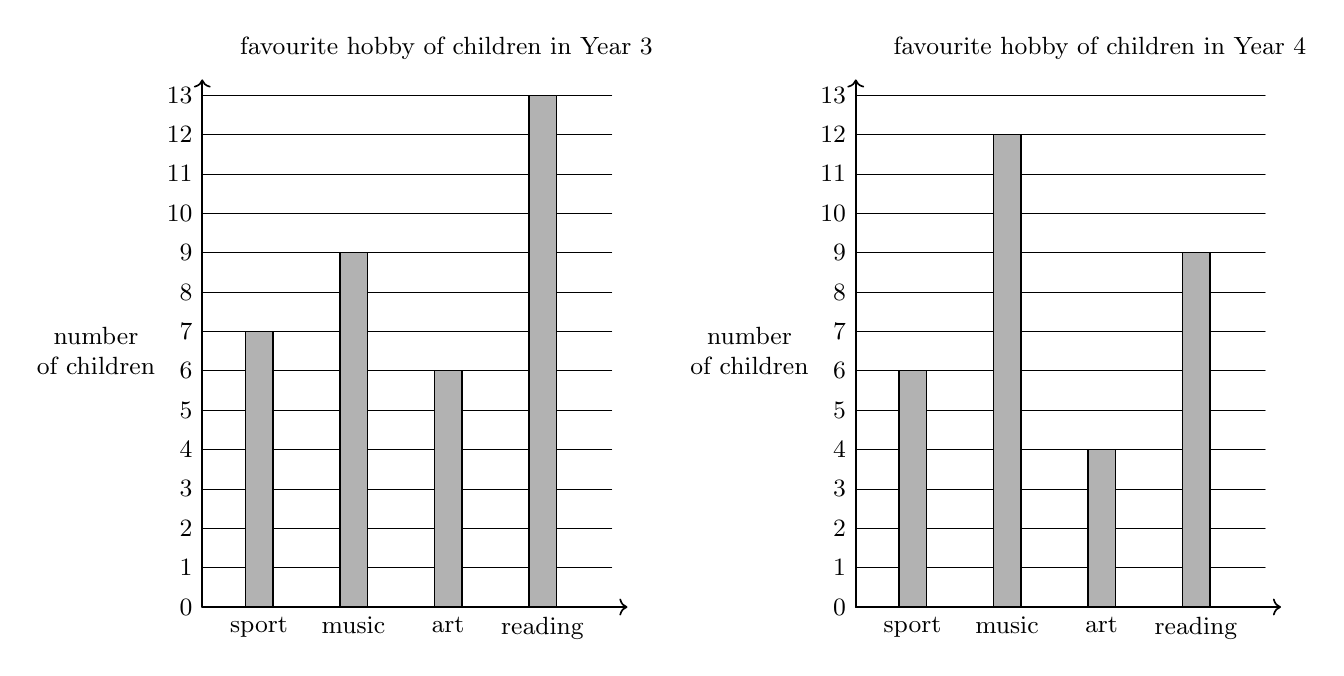
\begin{tikzpicture}[
			scale=1,
			every node/.style={font=\small, transform shape},
			line cap=round,
			line join=round
			]
			% Year 3 chart
			\begin{scope}[shift={(0,0)}]
				\node[align=center] at (3.1,7.1) {favourite hobby of children in Year 3};
				
				\draw[->, line width=0.6pt] (0,0) -- (0,6.7);
				\draw[->, line width=0.6pt] (0,0) -- (5.4,0);
				
				\foreach \y in {0,1,...,13}
				{
					\draw[line width=0.25pt] (0,\y/2) -- (5.2,\y/2);
					\node[left] at (0,\y/2) {\y};
				}
				
				\node[align=center] at (-1.35,3.25) {number\\of children};
				
				\fill[gray!60] (0.55,0) rectangle (0.9,3.5);
				\fill[gray!60] (1.75,0) rectangle (2.1,4.5);
				\fill[gray!60] (2.95,0) rectangle (3.3,3.0);
				\fill[gray!60] (4.15,0) rectangle (4.5,6.5);
				
				\draw[line width=0.5pt] (0.55,0) rectangle (0.9,3.5);
				\draw[line width=0.5pt] (1.75,0) rectangle (2.1,4.5);
				\draw[line width=0.5pt] (2.95,0) rectangle (3.3,3.0);
				\draw[line width=0.5pt] (4.15,0) rectangle (4.5,6.5);
				
				\node[below] at (0.72,0) {sport};
				\node[below] at (1.92,0) {music};
				\node[below] at (3.12,0) {art};
				\node[below] at (4.32,0) {reading};
			\end{scope}
			
			% Year 4 chart
			\begin{scope}[shift={(8.3,0)}]
				\node[align=center] at (3.1,7.1) {favourite hobby of children in Year 4};
				
				\draw[->, line width=0.6pt] (0,0) -- (0,6.7);
				\draw[->, line width=0.6pt] (0,0) -- (5.4,0);
				
				\foreach \y in {0,1,...,13}
				{
					\draw[line width=0.25pt] (0,\y/2) -- (5.2,\y/2);
					\node[left] at (0,\y/2) {\y};
				}
				
				\node[align=center] at (-1.35,3.25) {number\\of children};
				
				\fill[gray!60] (0.55,0) rectangle (0.9,3.0);
				\fill[gray!60] (1.75,0) rectangle (2.1,6.0);
				\fill[gray!60] (2.95,0) rectangle (3.3,2.0);
				\fill[gray!60] (4.15,0) rectangle (4.5,4.5);
				
				\draw[line width=0.5pt] (0.55,0) rectangle (0.9,3.0);
				\draw[line width=0.5pt] (1.75,0) rectangle (2.1,6.0);
				\draw[line width=0.5pt] (2.95,0) rectangle (3.3,2.0);
				\draw[line width=0.5pt] (4.15,0) rectangle (4.5,4.5);
				
				\node[below] at (0.72,0) {sport};
				\node[below] at (1.92,0) {music};
				\node[below] at (3.12,0) {art};
				\node[below] at (4.32,0) {reading};
			\end{scope}
		\end{tikzpicture}
	\end{center}
	
	\vspace{0.25cm}
	
	Naomi says,
	
	\vspace{0.25cm}
	
	\hspace*{1.5cm}`More children have music as a favourite hobby than reading.'
	
	\vspace{0.35cm}
	
	Naomi is not correct.
	
	\vspace{0.25cm}
	
	Explain why she is not correct.
	
	\vspace{0.3cm}
	
	\AnswerLine{16cm}
	
	\vspace{0.25cm}
	
	\AnswerLine{16cm}
	
	\vspace{0.25cm}
	
	\AnswerLine{16cm} \QuestionMarks{1}
	
	\vspace{0.8cm}
	
	\textbf{22}\quad
	Here are some fractions.
	
	\vspace{0.4cm}
	
	\[
	\frac{3}{14}
	\qquad\qquad
	\frac{2}{9}
	\qquad\qquad
	\frac{8}{14}
	\qquad\qquad
	\frac{9}{15}
	\qquad\qquad
	\frac{3}{21}
	\]
	
	\vspace{0.35cm}
	
	Draw a ring around the fraction that is equivalent to \(\dfrac{1}{7}\). \QuestionMarks{1}
	
	\vspace{0.8cm}
	
	\textbf{23}\quad
	Here is a Carroll diagram.
	
	\vspace{0.25cm}
	
	Some 2D shapes have been sorted on the diagram.
	
	\vspace{0.3cm}
	
	\begin{center}
		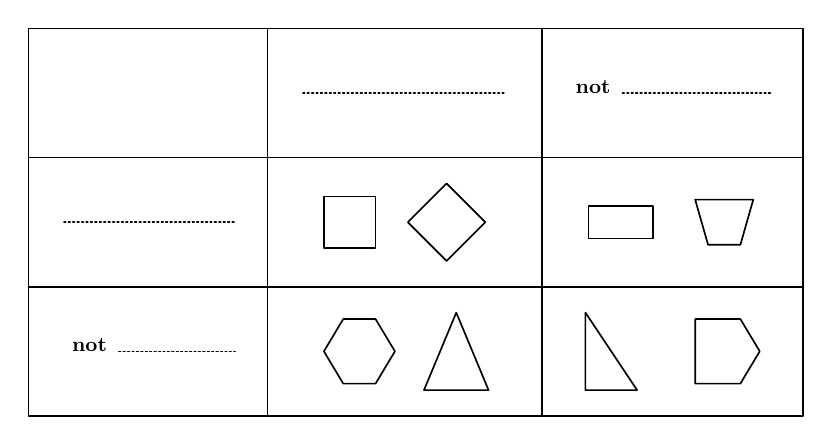
\begin{tikzpicture}[
			scale=0.82,
			every node/.style={font=\small, transform shape},
			line cap=round,
			line join=round
			]
			% Grid
			\draw[line width=0.6pt] (0,0) rectangle (12,6);
			\draw[line width=0.6pt] (3.7,0) -- (3.7,6);
			\draw[line width=0.6pt] (7.95,0) -- (7.95,6);
			\draw[line width=0.6pt] (0,2) -- (12,2);
			\draw[line width=0.6pt] (0,4) -- (12,4);
			
			% Heading blanks, vertically centered in header row
			\draw[densely dotted, line width=0.6pt] (4.25,5.0) -- (7.40,5.0);
			
			\node[anchor=base west] at (8.35,5.0) {\textbf{not}};
			\draw[densely dotted, line width=0.6pt] (9.2,5.0) -- (11.50,5.0);
			
			% Left column labels, vertically centered in their cells
			\draw[densely dotted, line width=0.6pt] (0.55,3.0) -- (3.20,3.0);
			
			\node[anchor=base west] at (0.55,1.0) {\textbf{not}};
			\draw[densely dotted, line width=0.6pt] (1.4,1.0) -- (3.20,1.0);
			
			% Row 1, column 1 shapes
			% Cell center: (5.825,3)
			\begin{scope}[shift={(5.825,3)}]
				\draw[line width=0.6pt]
				(-1.25,-0.40) rectangle (-0.45,0.40);
				
				\draw[line width=0.6pt]
				(0.65,0.60) -- (1.25,0) -- (0.65,-0.60) -- (0.05,0) -- cycle;
			\end{scope}
			
			% Row 1, column 2 shapes
			% Cell center: (9.975,3)
			\begin{scope}[shift={(9.975,3)}]
				\draw[line width=0.6pt]
				(-1.30,-0.25) rectangle (-0.30,0.25);
				
				\draw[line width=0.6pt]
				(0.35,0.35) -- (1.25,0.35) -- (1.05,-0.35) -- (0.55,-0.35) -- cycle;
			\end{scope}
			
			% Row 2, column 1 shapes
			% Cell center: (5.825,1)
			\begin{scope}[shift={(5.825,1)}]
				\draw[line width=0.6pt]
				(-1.25,0) --
				(-0.95,0.50) --
				(-0.45,0.50) --
				(-0.15,0) --
				(-0.45,-0.50) --
				(-0.95,-0.50) --
				cycle;
				
				\draw[line width=0.6pt]
				(0.30,-0.60) -- (0.80,0.60) -- (1.30,-0.60) -- cycle;
			\end{scope}
			
			% Row 2, column 2 shapes
			% Cell center: (9.975,1)
			\begin{scope}[shift={(9.975,1)}]
				\draw[line width=0.6pt]
				(-1.35,0.60) -- (-1.35,-0.60) -- (-0.55,-0.60) -- cycle;
				
				\draw[line width=0.6pt]
				(0.35,-0.50) --
				(1.05,-0.50) --
				(1.35,0) --
				(1.05,0.50) --
				(0.35,0.50) --
				cycle;
			\end{scope}
		\end{tikzpicture}
	\end{center}
	
	\vspace{0.25cm}
	
	Complete the headings for the Carroll diagram. \QuestionMarks{2}
	
	\vspace{0.8cm}
	
	\textbf{24}\quad
	Here is a coordinate grid.
	
	\vspace{0.25cm}
	
	There is a line drawn on the grid from point \(A\) to point \(B\).
	
	\vspace{0.3cm}
	
	\begin{center}
		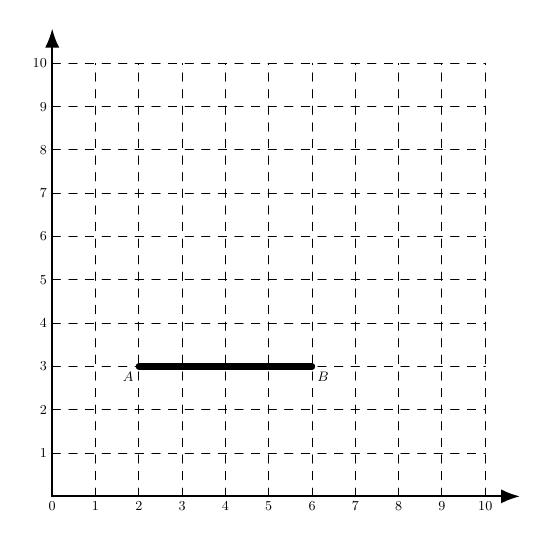
\begin{tikzpicture}[
			scale=0.55,
			every node/.style={font=\small, transform shape},
			line cap=round,
			line join=round
			]
			% Grid
			\draw[step=1, dashed, line width=0.35pt] (0,0) grid (10,10);
			
			% Axes
			\draw[-{Latex[length=2.4mm]}, line width=0.7pt] (0,0) -- (10.8,0);
			\draw[-{Latex[length=2.4mm]}, line width=0.7pt] (0,0) -- (0,10.8);
			
			% Axis labels
			\foreach \x in {0,1,...,10}
			\node[below] at (\x,0) {\x};
			
			\foreach \y in {1,2,...,10}
			\node[left] at (0,\y) {\y};
			
			% Line AB
			\draw[line width=2.3pt] (2,3) -- (6,3);
			\node[below left] at (2,3) {\(A\)};
			\node[below right] at (6,3) {\(B\)};
		\end{tikzpicture}
	\end{center}
	
	\vspace{0.3cm}
	
	Write the coordinates of point \(C\) and point \(D\) so that the points \(A\), \(B\), \(C\) and \(D\) can be joined to make a square.
	
	\vspace{0.55cm}
	
	\hfill
	\((\AnswerLine{2.2cm},\ \AnswerLine{2.2cm})\)
	\quad and \quad
	\((\AnswerLine{2.2cm},\ \AnswerLine{2.2cm})\)
	\QuestionMarks{1}
	
\end{document}